\chapter{ТЕОРЕТИЧЕСКОЕ ОБОСНОВАНИЕ СИСТЕМЫ, АРХИТЕКТУРА И РЕАЛИЗАЦИЯ}
\section{Модель мышления Марвина Мински}
\subsection{Крити-Селектор-Путь мышления}
В 2006 году Марвин Мински опубликовал свою книгу "The emotion machine" \cite{EmotionMachine}, в которой предложил свой взгляд на систему мышления и памяти человека. В основу теории легла парадигма триплета Критик-Селектор-Путь мышления, k-line для сопоставления знаний. На рисунке \ref{img:csw} представлена схематичное изображение Критика-Селектора-Пути мышления \\
\begin{figure} [h] 
  \center
  \includegraphics [scale=1.0] {CSW}
  \caption{Критик-Селектор-Путь мышления} 
  \label{img:csw}  
\end{figure}

\textbf{Критик} представляет собой определенный триггер: внешние обстоятельства, события или иное воздействие. Например, включился свет и зрачки сузились. Обожглись и одернули руку. Критик активируется только когда для этого достаточно обстоятельств. Одновременно могут активироваться несколько критиков. Например, человек решает сложную задачу. Идет активация множество критиков: считать, технические детали, кроме того параллельно может активироваться критик переработки, сообщающей о необходимости отдыха.\\
\textbf{Селектор} занимается выбором определенных ресурсов, которыми также являются Пути мышления. \\
\textbf{Путь мышления} это способ решения проблемы. Путь мышления также может активировать следующий критик. \\

На рисунке \ref{img:csw_ex} представления расширенная модель работы триплета Критик-Селектор-Путь мышления. Критик активирует селектор, который активирует путь мышления (синий круг). Путь мышления в свою очередь может активировать критик или же совершить определенные действия. Например, зажегся зеленый свет светофора, значит можно переходить дорогу. \\
Если активировалось много критиков, значит проблему нужно уточнить, так как степень неопределенности слишком высока. Если проблема очень похожа, то можно судить по аналогии.
\begin{figure} [h] 
  \center
  \includegraphics [scale=1.0] {CSW_EX}
  \caption{Критик-Селектор-Путь мышления в разрезе ресурсов} 
  \label{img:csw_ex}  
\end{figure}

\subsection{Уровни мышления}
Концепция уровней мышления представляет собой степень ментальной активности человека. Никто из людей не может похвастаться скоростью гепарда, гибкости кошки, силой медведя. Но наш вид все это компенсирует возможностью изобретения путей мышления. Например, чтобы быть быстрыми мы изобрели самолеты, машины. Чтобы быть сильными, мы изобрели оружие. Что же делает это возможным? Безусловно результатом всего является взаимодействие человека с окружающим миром. Именно данное взаимодействие заставляет людей изобретать что-то новое, создавать шедевры литературы и летать в космос. Но как же мы всего этого добиваемся начиная от, инстинктивного одергивая руки до создания Теории всего \cite{Hawking}. Далее мы рассмотрим концепцию уровней мышления.
\begin{enumerate}
	\item Инстинктивный уровень
	\item Уровень обученных реакций
	\item Уровень рассуждений
	\item Рефлексивный уровень
	\item Саморефлексивный уровень
	\item Самосознательный уровень
\end{enumerate}
\textbf{Инстинктивный уровень.} На данном уровне происходят инстинктивные реакции (врожденные). Например, боязнь обжечься. Не прыгать под машину. Общую формулу для этого уровня можно выразить как "Если ..., то сделать так".\\
\textbf{Уровень обученных реакций.} На  данной уровне происходит мышление обученных реакций, то есть тех реакций, которыми человек обучается в течение жизни. Например, переходить дорогу на зеленых свет. Общую формулу для этого уровня можно выразить как "Если ..., то сделать так". \\
\textbf{Уровень рассуждений.} На  данной уровне происходит мышление с использованием рассуждений. Если я сделаю так, то будет ... Например, если перебежать дорогу на зеленый свет, то можно успеть вовремя. На данном уровне сравниваются последствия нескольких решений и выбирается оптимальное. Общую формулу для этого уровня можно выразить как "Если ..., то сделать так, тогда будет так". \\
\textbf{Рефлексивный уровень.} На данном уровне происходит рассуждение с учетом анализа прошлых событий. Например, прошлый раз я побежал на моргающий зеленый и чуть не попал под машину.\\
\textbf{Саморефлексивный уровень.} На данном уровне происходит оценка себя. Строится определенная модель с помощью которой идет оценка своих поступков. Например, мое решение не пойти на это собрание было неверным, так как я упустил столько возможностей, я был \textbf{легкомысленный}.\\
\textbf{Самосознательный уровень.} Самозонательный уровень на данный момент характерен только для человека. На данном уровне идет оценка поступков человека с точки зрения высших идеалов и внешних оценок. Например, а что подумают мои друзья? А как бы поступил мой герой? \\
Деление на данные уровне носит условный характер. Например уровень 5 и 6 можно объединить. Но по словам Марвина Мински принцип бритвы Оккама успешно применяется в физики, но в психологии он не должен применяться также легко. \\
На рисунке \ref{img:thinkinglevels} представлена схематичное изображение уровней мышления. 1-3 уровни составляют личность человека. 2-5 представляют ЭГО человека (Человеческое Я) - осознание человека в общении с окружающими. 3-6 представляют собой сверх ЭГО человека (сверх Я) - его моральные установки.
\begin{figure} [h] 
  \center
  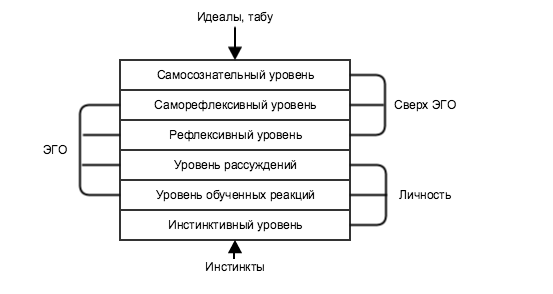
\includegraphics [scale=1.0] {thinkinglevels}
  \caption{Критик-Селектор-Путь мышления в разрезе ресурсов} 
  \label{img:thinkinglevels}  
\end{figure}

%\newpage
%============================================================================================================================




\clearpage